\begin{enumerate}[label=\thechapter.\arabic*,ref=\thechapter.\theenumi]

\item Consider the differential equation $\frac{d^2y}{dx^2}-2\frac{dy}{dx}+y=0$. The boundary conditions are $y=0$ and $\frac{dy}{dx}=1$ at $x=0$. Then the value of $y$ at $x=\frac{1}{2}$ \hfill (GATE AE 2022)\\
\solution
\iffalse
\let\negmedspace\undefined
\let\negthickspace\undefined
\documentclass[journal,12pt,twocolumn]{IEEEtran}
\usepackage{cite}
\usepackage{amsmath,amssymb,amsfonts,amsthm}
\usepackage{algorithmic}
\usepackage{graphicx}
\usepackage{textcomp}
\usepackage{xcolor}
\usepackage{txfonts}
\usepackage{listings}
\usepackage{enumitem}
\usepackage{mathtools}
\usepackage{gensymb}
\usepackage{comment}
\usepackage[breaklinks=true]{hyperref}
\usepackage{tkz-euclide} 
\usepackage{listings}
\usepackage{gvv}                                        
\def\inputGnumericTable{}                                 
\usepackage[latin1]{inputenc}                                
\usepackage{color}                                            
\usepackage{array}                                            
\usepackage{longtable}                                       
\usepackage{calc}                                             
\usepackage{multirow}                                         
\usepackage{hhline}                                           
\usepackage{ifthen}                                           
\usepackage{lscape}
\newtheorem{theorem}{Theorem}[section]
\newtheorem{problem}{Problem}
\newtheorem{proposition}{Proposition}[section]
\newtheorem{lemma}{Lemma}[section]
\newtheorem{corollary}[theorem]{Corollary}
\newtheorem{example}{Example}[section]
\newtheorem{definition}[problem]{Definition}
\newcommand{\BEQA}{\begin{eqnarray}}
\newcommand{\EEQA}{\end{eqnarray}}
\newcommand{\define}{\stackrel{\triangle}{=}}
\theoremstyle{remark}
\newtheorem{rem}{Remark}
\begin{document}

\bibliographystyle{IEEEtran}
\vspace{3cm}

\title{GATE: AE - 37.2022}
\author{EE23BTECH11224 - Sri Krishna Prabhas Yadla$^{*}$% <-this % stops a space
}
\maketitle
\newpage
\bigskip

\renewcommand{\thefigure}{\arabic{figure}}
\renewcommand{\thetable}{\arabic{table}}


\vspace{3cm}
\textbf{Question:} Consider the differential equation $\frac{d^2y}{dx^2}-2\frac{dy}{dx}+y=0$. The boundary conditions are $y=0$ and $\frac{dy}{dx}=1$ at $x=0$. Then the value of $y$ at $x=\frac{1}{2}$ \hfill (GATE AE 2022)\\
\solution
\fi
\begin{table}[htbp]
	\centering
	\def\arraystretch{1.5}
	\begin{tabular}{|c|c|c|}
\hline
\textbf{Parameters} & \textbf{Values} & \textbf{Description} \\
\hline
$y(0)$ & 0 & $y$ at $x=0$\\
\hline
$y'(0)$& 1 &$\frac{dy}{dx}$ at $x=0$ \\
\hline
\end{tabular}

	\caption{Parameters}
	\label{tab:parameters}
\end{table}
\begin{align}
\label{L(y'')}\frac{d^2y}{dx^2} &\system{L} s^2Y(s)-sy(0)-y'(0)\\
\label{L(y')}\frac{dy}{dx} &\system{L} sY(s)-y(0)
\end{align}
Applying Laplace Transform, using \eqref{L(y'')} and \eqref{L(y')},
\begin{align}
s^2Y(s)-sy(0)-y'(0) - 2(sY(s)-y(0)) + Y(s) = 0
\end{align}
From \tabref{tab:parameters},
\begin{align}
(s^2-2s+1)Y(s)-1 &= 0 \\
Y(s) &= \frac{1}{(s-1)^2}\\
\label{L(t^n)}t^n &\system{L} \frac{n!}{s^{n+1}}\\
	\label{complex_shift}e^{at} x(t) &\system{L} X(s-a)
\end{align}
Taking Inverse Laplace Transform for $Y(s)$, using \eqref{L(t^n)} and \eqref{complex_shift},
\begin{align}
y(x) &= xe^x \\
\implies y\brak{\frac{1}{2}} &= \frac{\sqrt{e}}{2}
\end{align}
\begin{figure}[htbp]
	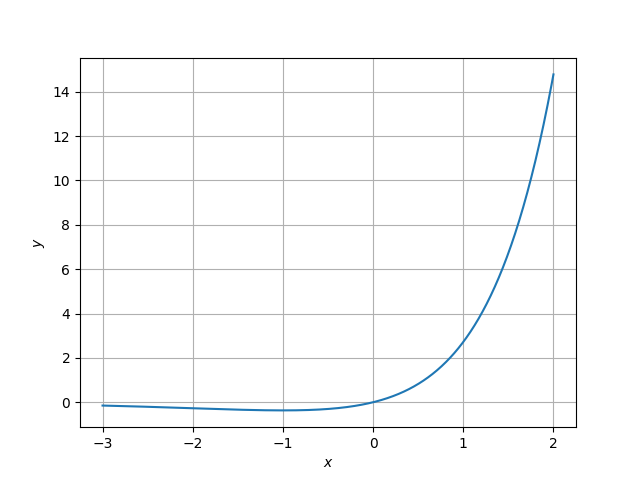
\includegraphics[width=\columnwidth]{2022/AE/37/figs/plot.png}
	\caption{Plot of $y(x)$}
	\label{fig:plot}
\end{figure}

\pagebreak

\item  A process described by the transfer function
\begin{align}
    G_p(s) = \frac{\brak{10s+1}}{\brak{5s+1}} \nonumber
\end{align}
is forced by a unit step input at time $t = 0$. The output value immediately after the unit step input (at $t = 0^+$) is ? \hfill(Gate 2022 CH 34)\\
\solution
\iffalse
\documentclass[journal,12pt,twocolumn]{IEEEtran}
\usepackage{cite}
\usepackage{amsmath,amssymb,amsfonts,amsthm}
\usepackage{algorithmic}
\usepackage{graphicx}
\usepackage{textcomp}
\usepackage{xcolor}
\usepackage{txfonts}
\usepackage{listings}
\usepackage{enumitem}
\usepackage{mathtools}
\usepackage{gensymb}
\usepackage{comment}
\usepackage[breaklinks=true]{hyperref}
\usepackage{tkz-euclide}
\usepackage{listings}
\usepackage{gvv}
\def\inputGnumericTable{}
\usepackage[latin1]{inputenc}
\usepackage{color}
\usepackage{array}
\usepackage{longtable}
\usepackage{calc}
\usepackage{multirow}
\usepackage{hhline}
\usepackage{ifthen}
\usepackage{lscape}
\usepackage{caption}

\newtheorem{theorem}{Theorem}[section]
\newtheorem{problem}{Problem}
\newtheorem{proposition}{Proposition}[section]
\newtheorem{lemma}{Lemma}[section]
\newtheorem{corollary}[theorem]{Corollary}
\newtheorem{example}{Example}[section]
\newtheorem{definition}[problem]{Definition}
\newcommand{\BEQA}{\begin{eqnarray}}
\newcommand{\EEQA}{\end{eqnarray}}
\newcommand{\define}{\stackrel{\triangle}{=}}
\theoremstyle{remark}
\newtheorem{rem}{Remark}
\begin{document}

\bibliographystyle{IEEEtran}
\vspace{3cm}

\title{GATE: CH - 34.2022}
\author{EE23BTECH11010 - Venkatesh D Bandawar $^{*}$% <-this % stops a space
}
\maketitle
% \newpage
\bigskip

% \renewcommand{\thefigure}{\theenumi}
% \renewcommand{\thetable}{\theenumi}

\textbf{Question:} A process described by the transfer function
\begin{align}
    G_p(s) = \frac{\brak{10s+1}}{\brak{5s+1}} \nonumber
\end{align}
is forced by a unit step input at time $t = 0$. The output value immediately after the unit step input (at $t = 0^+$) is ? \hfill(Gate 2022 CH 34)\\
\solution
\fi
\begin{table}[!h] 
\centering
\begin{tabular}{|c|c|}
\hline
     \textbf{Parameters}&\textbf{Description}  \\
     \hline
     $X(s)$ & Laplace transform of $x(t)$ \\
     \hline
     $Y(s)$ & Laplace transform of $y(t)$ \\
     \hline
     $G_p(s) = \frac{Y(s)}{X(s)}$ & Transfer function\\
     \hline
     $x(t) = u(t)$ & unit step function\\
     \hline
\end{tabular}

\caption{Given parameters}
\label{given parameters list.gate.2022.ch.34}
\end{table}
\begin{align}
    G_p(s) = \frac{Y(s)}{X(s)} &= \frac{\brak{10s+1}}{\brak{5s+1}}\\
    u(t) \system{\mathcal{L}} \frac{1}{s} \label{laplace transform of unit function 2022.ch.34}
\end{align}
From equation \eqref{laplace transform of unit function 2022.ch.34}:
\begin{align}
    Y(s) &= \frac{\brak{10s+1}}{s\brak{5s+1}}\\
    &= \frac{1}{s} + \frac{5}{5s+1}
\end{align}
Taking inverse laplace transformation, 
\begin{align}
    \frac{1}{s} &\mathrel{\substack{\mathcal{L}^{-1}\\\longleftrightarrow}} u(t)\\
    \frac{1}{s-c} &\mathrel{\substack{\mathcal{L}^{-1}\\\longleftrightarrow}} e^{ct} u(t)
\end{align}
\begin{align}
    y(t) &= \brak{1 + e^{\frac{-t}{5}}}u(t)\\
    y(0^+) &= 2
\end{align}

\begin{figure}[!h] 
    \centering
    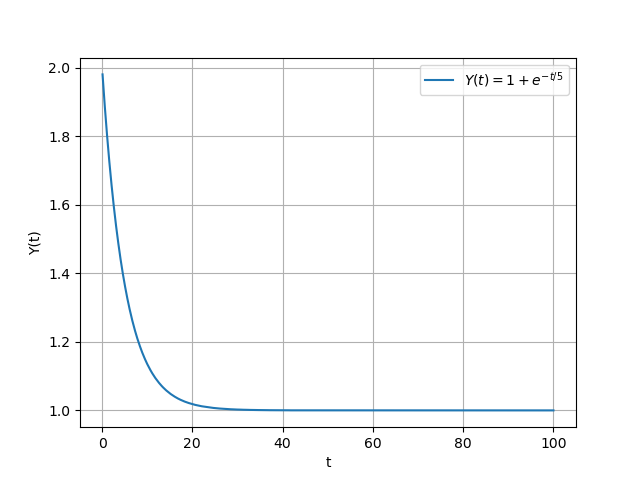
\includegraphics[width=\columnwidth]{2022/CH/34/figs/Graph_of_y(t).png}
    \caption{Graph of y(t)}
    \label{fig:Graph1_gate_CE_30}
    \end{figure}


\pagebreak
\item The transfer function of a real system $H(S)$ is given as:
\begin{align}
    H(s) = \frac{As + B}{s^2 + Cs + D}\nonumber
\end{align}
where $A, B, C$ and $D$ are positive constants. This system cannot operate as
\begin{enumerate}[label={(\Alph*)}]
    \item Low pass filter
    \item High pass filter
    \item Band pass filter
    \item An Integrator
\end{enumerate}\hfill(GATE EE 11 2022)

\solution
 \iffalse
\let\negmedspace\undefined
\let\negthickspace\undefined
\documentclass[journal,12pt,twocolumn]{IEEEtran}
\usepackage{cite}
\usepackage{amsmath,amssymb,amsfonts,amsthm}
\usepackage{algorithmic}
\usepackage{graphicx}
\usepackage{textcomp}
\usepackage{xcolor}
\usepackage{txfonts}
\usepackage{listings}
\usepackage{enumitem}
\usepackage{mathtools}
\usepackage{gensymb}
\usepackage{comment}
\usepackage[breaklinks=true]{hyperref}
\usepackage{tkz-euclide} 
\usepackage{listings}
\usepackage{gvv} 
\usepackage{caption}
\def\inputGnumericTable{}                   

%\usepackage[latin1]{inputenc}                                
\usepackage{color}                                            
\usepackage{array}                                            
\usepackage{longtable}                                       
\usepackage{calc}                                             
\usepackage{multirow}                                         
\usepackage{hhline}                                           
\usepackage{ifthen}                                           
\usepackage{lscape}
\usepackage{tikz}
\newtheorem{theorem}{Theorem}[section]
\newtheorem{problem}{Problem}
\newtheorem{proposition}{Proposition}[section]
\newtheorem{lemma}{Lemma}[section]
\newtheorem{corollary}[theorem]{Corollary}
\newtheorem{example}{Example}[section]
\newtheorem{definition}[problem]{Definition}
\newcommand{\BEQA}{\begin{eqnarray}}
\newcommand{\EEQA}{\end{eqnarray}}
\newcommand{\define}{\stackrel{\triangle}{=}}
\theoremstyle{remark}
\newtheorem{rem}{Remark}

\begin{document}

\bibliographystyle{IEEEtran}
\vspace{3cm}

\title{GATE: EE - 11.2022}
\author{EE23BTECH11013 - Avyaaz$^{*}$% <-this % stops a space 
}
\maketitle
\newpage
\bigskip

\renewcommand{\thefigure}{\arabic{figure}}
\renewcommand{\thetable}{\arabic{table}}

\large\textbf{\textsl{Question:}}
The transfer function of a real system $H(S)$ is given as:
\begin{align}
    H(s) = \frac{As + B}{s^2 + Cs + D}\nonumber
\end{align}
where $A, B, C$ and $D$ are positive constants. This system cannot operate as
\begin{enumerate}[label={(\Alph*)}]
    \item Low pass filter
    \item High pass filter
    \item Band pass filter
    \item An Integrator
\end{enumerate}\hfill(GATE EE 11 2022) \\
\solution
\fi
The transfer function $H(s)$ is given by: 
\begin{align}
    H(s) = \frac{As + B}{s^2 + Cs + D}\label{eq:given.EE.11.2022}
\end{align}
Put $s = j\omega$ in \eqref{eq:given.EE.11.2022}:
\begin{align}
    H(j\omega) = \frac{A(j\omega) + B}{(j\omega)^2 + C(j\omega) + D} \\
    |H(j\omega)| = \frac{\sqrt{(A\omega)^2 + B^2}}{\sqrt{(D - \omega^2)^2 + (\omega C)^2}}\label{eq:magnitude.EE.11.2022}
\end{align}


\begin{table}[htbp]
\setlength{\extrarowheight}{4pt}
\setlength{\tabcolsep}{3pt}
\centering
\begin{tabular}{|c|c|}
\hline
\textbf{Parameter} & \textbf{Description}\\
\hline 
Low Pass Filter & The gain should be finite at low frequency  \\
\hline
High Pass Filter &The gain should be finite at high frequency \\
\hline
Band Pass Filter& Finite gain over frequency band \\
\hline
Integrator & Transfer function should have at least\\& one pole at origin \\
\hline
\end{tabular}

\caption{Conditions}
\label{tab:inputs.EE.11.2022}
\end{table}
% \item \noindent From \tabref{tab:inputs.EE.11.2022} and equation \eqref{eq:magnitude.EE.11.2022}:
\begin{enumerate}[label={\alph*)}]
    \item Low Pass Filter:
    
  At low frequency $(\omega = 0 )$:
 \begin{align}
     |H(\omega = 0)| = \frac{B}{D}\label{eq:lowpass.EE.11.2022}
 \end{align}
$\therefore$ H(s) can operate as Low pass filter.

\item High Pass Filter:

% From \tabref{tab:inputs.EE.11.2022} and equation \eqref{eq:magnitude.EE.11.2022}:

At high frequency $(\omega = \infty )$:
 \begin{align}
     |H(\omega = \infty)| = 0 \label{eq:highpass.EE.11.2022}
 \end{align}
 % From \tabref{tab:inputs.EE.11.2022}:
 
$\therefore$ $H(s)$ cannot operate as High pass filter.
\item Band Pass Filter:

 Assuming B is a very less positive valued constant as compared to others:
\begin{align}
        |H(j\omega)| = \frac{(A\omega)}{\sqrt{(D - \omega^2)^2 + (\omega C)^2}}\\
   \implies      |H(\omega = 0)| = 0 \text{ and }  |H(\omega = \infty)| = 0 \label{eq:bandpass.EE.11.2022}
\end{align}

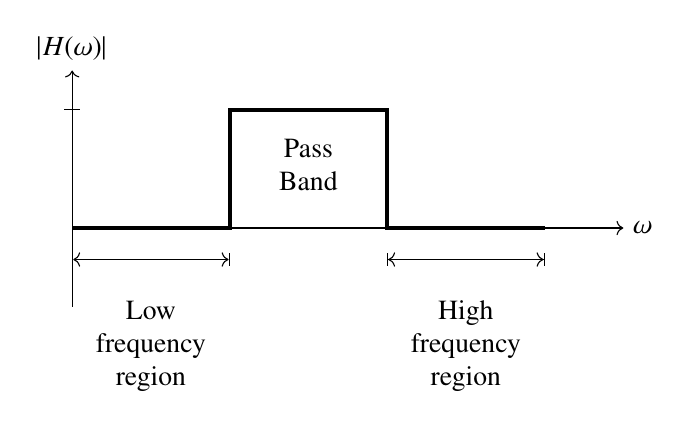
\begin{tikzpicture}
  
    \draw[->] (0,0) -- (7,0) node[right] {$\omega$};
   
    \draw[->] (0,-1) -- (0,2) node[above] {$|H(\omega)|$};
  
    \draw[line width=1.5pt]  (0,0) -- (2,0) -- (2,1.5) -- (4,1.5) -- (4,0) --(6,0);
    \draw[-]{(0,1.5)};
      \draw (-0.1,1.5) -- (0.1,1.5);
         \draw[|<->|]{(0,-0.4) -- (2,-0.4)};
    \node[align=center] at (1,-1.5) {Low \\frequency\\ region};
         \draw[| <-> |]{(4,-0.4) -- (6,-0.4)};
    \node[align=center] at (5,-1.5) {High \\frequency\\ region};
    \node[align=center] at (3,0.8) {Pass\\Band};

\end{tikzpicture}
$\because$ $H(s)$ passes frequency between low and high frequencies.

$\therefore$ $H(s)$ can operate as a band pass filter.
\item Integrator:

At very high value of frequency$(\omega\mkern-4mu \rightarrow\mkern-6mu\infty)$:
\begin{align}
    H(s) \approx \frac{As}{s^2} \approx \frac{A}{s}\label{eq:integrator.EE.11.2022}
\end{align}
From \tabref{tab:inputs.EE.11.2022}:

$\therefore$ $H(s)$ can operate as an Integrator.
\end{enumerate}
% From equations \eqref{eq:lowpass.EE.11.2022},\eqref{eq:highpass.EE.11.2022},\eqref{eq:bandpass.EE.11.2022} and \eqref{eq:integrator.EE.11.2022}:

% The Transfer function $H(s)$ cannot be operated as a High pass filter.
% \begin{figure}[htbp]
%     \centering
%     \includegraphics[width = \columnwidth]{}
%   \caption{}
%     \label{fig:graph1}
% \end{figure}

% \bibliographystyle{IEEEtran}
%\end{document}

\pagebreak

\item In a circuit, there is a series connection of an ideal resistor and an ideal capacitor.
The conduction current (in Amperes) through the resistor is $2\sin\brak{t + \frac{\pi}{2}}$. The displacement current (in Amperes) through the capacitor is \rule{1cm}{0.15mm}.\\ 
\begin{enumerate}[label=(\Alph*)]
    \item $2\sin\brak{t}$
    \item $2\sin\brak{t+\pi}$
    \item $2\sin\brak{t +\frac{\pi}{2}}$
    \item $0$
\end{enumerate}
\hfill(GATE 2022 EC 24)\\
\solution
\iffalse
\documentclass[journal,12pt,twocolumn]{IEEEtran}
\usepackage{amsmath,amssymb,amsfonts,amsthm}
\usepackage{txfonts}
\usepackage{tkz-euclide}
\usepackage{listings}
\usepackage{gvv}
\usepackage[latin1]{inputenc}
\usepackage{adjustbox}
\usepackage{array}
\usepackage{tabularx}
\usepackage{enumitem}
\usepackage{pgf}
\usepackage{lmodern}
\usepackage{circuitikz}
\usepackage{tikz}
\usepackage{graphicx}


\begin{document}
\bibliographystyle{IEEEtran}

\vspace{3cm}

\title{}
\author{EE23BTECH11054 -  Sai Krishna Shanigarapu$^{*}$
}
\maketitle
\newpage
\bigskip

% \renewcommand{\thefigure}{\theenumi}
% \renewcommand{\thetable}{\theenumi}

\section*{Gate EC 2022}
54. \hspace{2pt}In a circuit, there is a series connection of an ideal resistor and an ideal capacitor.
The conduction current (in Amperes) through the resistor is $2\sin\brak{t + \frac{\pi}{2}}$. The displacement current (in Amperes) through the capacitor is \rule{1cm}{0.15mm}.\\ 
\begin{enumerate}[label=(\Alph*)]
    \item $2\sin\brak{t}$
    \item $2\sin\brak{t+\pi}$
    \item $2\sin\brak{t +\frac{\pi}{2}}$
    \item $0$
\end{enumerate}
\hfill(GATE EC 2022)

\solution
\fi
\begin{table}[ht]
       \setlength{\arrayrulewidth}{0.3mm}
\setlength{\tabcolsep}{20pt}
\renewcommand{\arraystretch}{1.5}

\begin{tabular}{|c|c|c|}
\hline
Parameter& Description & Value\\
\hline
$I_c$ & Conduction Current & $2\sin\brak{t + \frac{\pi}{2}}$\\
\hline
%$I_d$ & Displacement current & ?\\
%\hline
$A$ & Cross-sectional area & \\
\hline
\end{tabular}

    \caption{Parameters}
    \label{tab:tab_gate_ec_2022_24_1}
\end{table}


\begin{table}[ht]
       \setlength{\arrayrulewidth}{0.3mm}
\setlength{\tabcolsep}{20pt}
\renewcommand{\arraystretch}{1.5}

\begin{tabular}{|c|c|c|}
\hline
Parameter & Description & Formula\\
\hline
$Q$ & Charge & $\int I_c\, dt$\\
\hline
$D$ & Electric Displacement & $\frac{Q}{A}$\\ 
\hline
$J_D$ & Displacement current density & $\frac{\partial D}{\partial t}$\\
\hline
$I_D$ & Displacement current & $J_D\text{ x }A$\\
\hline




\end{tabular}

    \caption{Formulae}
    \label{tab:tab_gate_ec_2022_24_2}
\end{table}

\begin{table}[ht]
       \setlength{\arrayrulewidth}{0.3mm}
\setlength{\tabcolsep}{20pt}
\renewcommand{\arraystretch}{1.5}



\begin{tabular}{|c|c|}
\hline

S Domain & Time Domain\\
\hline
$\frac{1}{s}$ & $u\brak{t}$\\
\hline
$\frac{-s}{a^2+s^2}$ & $-\cos\brak{at}$\\
\hline
$\frac{a}{a^2+s^2}$ & $\sin\brak{at}$\\
\hline
$\frac{1}{s+a}$ & $e^{-at}$\\
\hline

\end{tabular}


    \caption{Laplace transforms}
    \label{tab:tab_gate_ec_2022_24_3}
\end{table}

\begin{align}
    \mathcal{L}\sbrak{\int f\brak{t}\, dt} &= \int_{0}^{\infty}\sbrak{\int f\brak{t}\, dt}e^{-st}\, dt\\
    &= \int_{0}^{\infty}u\, dv \quad \text{where}\begin{cases}
  u =\int f\brak{t}dt \\
  dv  =e^{-st}dt
\end{cases}\\
&= uv - v\int du\\
&= \frac{1}{s}\int f\brak{t}dt|_0 + \frac{1}{s}\int_{0}^{\infty}f\brak{t}e^{-st}dt\\
&\implies \frac{1}{s}\int f\brak{t}dt|_0 + \frac{1}{s}F\brak{s} \label{eq:eq_gate_ec_2022_24_1}
\end{align}


\begin{figure}[ht]
  \centering
      \begin{circuitikz}[american]
\draw (0,3) to [short,*-, i=$i_c$] (1,3) to [R=$R$] (4,3);
\draw (0,0) to [short, *-] (4,0);
\draw (4,3) to [short, i=$i_d$] (4,2.5) to [C=$C$] (4,0);
\end{circuitikz}
  \caption{Circuit 1}
\end{figure}

From Table \ref{tab:tab_gate_ec_2022_24_2}, Table \ref{tab:tab_gate_ec_2022_24_3} and eq (\ref{eq:eq_gate_ec_2022_24_1})
\begin{align}
    I_c\brak{s} &= \frac{2s}{s^2 + 1}\\
    Q_c\brak{s} &= \frac{2}{s\brak{s^2 + 1}}\\
    D\brak{s} &= \frac{1}{A}\brak{\frac{2}{s\brak{s^2 + 1}}}\\
    J_D\brak{s} &= \frac{2}{A}\brak{\frac{1}{s^2 + 1}}\\
    I_D\brak{s} &= \frac{2}{s^2 + 1}\\
    \implies I_D &= 2\sin{t}
\end{align}


\begin{figure}[ht]
  \centering
      \begin{tikzpicture}

        \draw[->] (-0.5,0) -- (4.5,0) node[right]{$E_{\text{ref}}$};
        \draw[->] (0,-0.5) -- (0,4.5) node[above]{$J_d$};
        

        \draw (0,0) -- (4,4);
        

        \draw[dashed] (4,0) -- (4,4);
        \node[right] at (4,4) {$\overline{J}$};
        \draw[dotted] (4,4) -- (4,0) node[below]{$J_c$};

        \draw[dashed] (0,4) -- (4,4);
        \draw[dotted] (4,4) -- (0,4) node[left]{$J_d$};
        

        \draw[->] (0.5,0) arc (0:90:0.5);
        \node[right] at (0.5,0.3) {$\frac{\pi}{2}$};
\end{tikzpicture}


  \caption{Phasor plot}
  \label{fig:fig_gate_ec_2022_24_1}
\end{figure}

From figure \ref{fig:fig_gate_ec_2022_24_1}, phase of $I_d$ is $\frac{\pi}{2}$

\begin{align}
    \therefore I_d = 2\sin\brak{t + \frac{\pi}{2}}
\end{align}
$\therefore$ (C) is correct.


\begin{figure}[ht]
    \centering
    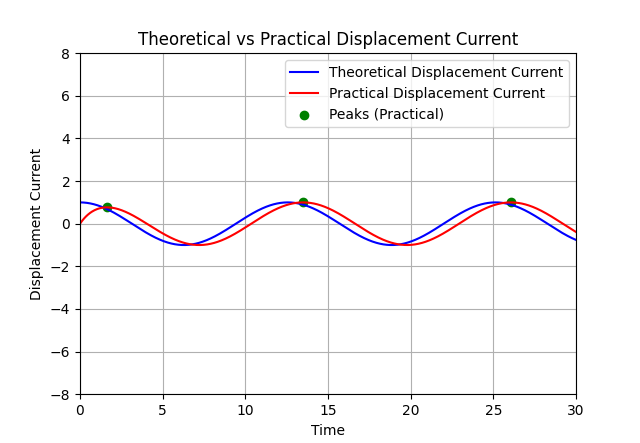
\includegraphics[width=\columnwidth]{2022/EC/24/figs/Figure_2.png}
    \caption{Thoritical vs Practical simulation}
    \label{fig:fig_gate_ec_2022_24_2}
\end{figure}

\begin{figure}[ht]
    \centering
    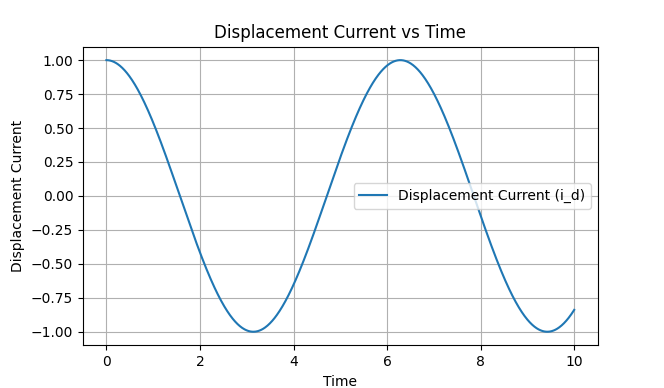
\includegraphics[width=\columnwidth]{2022/EC/24/figs/Figure_4.png}
    \caption{Displacement current}
    \label{fig:fig_gate_ec_2022_24_3}
\end{figure}



%\end{document}

\end{enumerate}
